  %% ACM sigconf: full two-column research report (nonacm). Build:  pdflatex bimodal_report  (x2)
  \documentclass[sigconf,nonacm]{acmart}
  \usepackage{amsmath}
  \usepackage{booktabs}
  \usepackage[english]{babel}
  \usepackage{balance}
  \usepackage{microtype}
  \usepackage{graphicx}
  \usepackage{xurl}
  % Self-contained for Overleaf: all generated evaluation values are inlined below.
  % Per-class qualitative thumbnails live under eval_output/qual_images/ ; upload
  % that folder to Overleaf alongside this file to render Table~\ref{tab:qualimages}.
  \graphicspath{{eval_output/}{./}}

  % Course submission: no permission footnote
  \renewcommand\footnotetextcopyrightpermission[1]{}
  \settopmatter{printacmref=false,printfolios=true}

  % --- title & authors (edit names/emails before submission if desired) ---
  \title[Bimodal Affective Alignment]{Bimodal Affective Alignment: Enhancing Conversational Empathy through Textual and Facial Fusion}

  \author{Sainadth Pagadala}
  \email{spagadala1@islander.tamucc.edu}
  \affiliation{%
    \department{College of Engineering and Computer Science}
    \institution{Texas A\&M University--Corpus Christi}
    \city{Corpus Christi}
    \state{TX}
    \postcode{78412}
    \country{USA}}
  \author{Minhua Huang}
  \authornote{Course instructor and project advisor.}
  \email{minhua.huang@tamucc.edu}
  \affiliation{%
    \department{College of Engineering and Computer Science}
    \institution{Texas A\&M University--Corpus Christi}
    \city{Corpus Christi}
    \state{TX}
    \postcode{78412}
    \country{USA}}

  \renewcommand{\shortauthors}{Pagadala and Huang}

  % CCS 2012
\begin{CCSXML}
<ccs2012>
<concept>
  <concept_id>10003120.10003121</concept_id>
  <concept_desc>Human-centered computing~Human computer interaction (HCI)</concept_desc>
  <concept_significance>500</concept_significance>
</concept>
<concept>
  <concept_id>10010147.10010257.10010293.10010294</concept_id>
  <concept_desc>Computing methodologies~Neural networks</concept_desc>
  <concept_significance>300</concept_significance>
</concept>
</ccs2012>
\end{CCSXML}
  \ccsdesc[500]{Human-centered computing~Human computer interaction (HCI)}
  \ccsdesc[300]{Computing methodologies~Neural networks}

  \keywords{affective computing, emotion recognition, multimodal fusion, GoEmotions, FER, FLAN-T5, dialogue}

  \begin{document}
  \begin{abstract}
  Conversational systems that read only one channel of human affect often misread the situation: text can hide what a person is feeling, and a face can contradict the words. This work builds and evaluates a bimodal pipeline that listens to both at once. A RoBERTa text classifier (fine-tuned on GoEmotions) and a ResNet-50 face classifier (FER2013-aligned) each emit a seven-way affect distribution, and a single trust weight $\alpha\in[0,1]$ fuses them via
  $b^*=\arg\max_k\bigl(\alpha P_\text{text}(k)+(1\!-\!\alpha)P_\text{face}(k)\bigr)$.
  The fused class together with the user's utterance feeds FLAN--T5, which produces a short empathetic reply. A Streamlit interface exposes both probability vectors, the fused decision, an explicit affective-dissonance flag, and per-stage timings, so a reviewer can see -- not just trust -- how the system is reasoning. We report unimodal and fused accuracy on the full GoEmotions and FER2013 test splits, a FER2013 fine-tune that lifts visual top-1 from 23.1\% to 68.5\%, real-image and synthetic dissonance evaluations, and a latency breakdown. Affect inference takes about 40\,ms on Apple MPS -- well inside the 400\,ms Doherty threshold -- while end-to-end response generation with FLAN--T5 (base) lands at 955\,ms.
  \end{abstract}

  \maketitle

  \section{Introduction}
  \subsection{Problem and motivation}
  When a dialogue system has to infer affect from text alone it is easy to fool: a sarcastic remark looks happy on the surface, a polite ``I'm fine'' hides distress, and a deadpan one-liner gives almost no signal at all. Vision alone has the symmetric weakness -- the same neutral face appears in good lighting, bad lighting, off-axis, or partly occluded. In either case the system has to guess, and a wrong guess in the empathy loop erodes user trust quickly~\cite{card1983human}. Reading both channels at once, when they are available, gives the model a second opinion and -- equally important -- a way to flag the cases where the two opinions disagree.

  \subsection{Related work}
  \paragraph{Multimodal emotion recognition.} Fusing language with facial or vocal cues is a long-standing line of work in affective computing~\cite{picard1997affective,baltrusaitis2019multimodal}. Natural multimodal corpora such as IEMOCAP~\cite{busso2008iemocap}, CMU-MOSEI~\cite{zadeh2018mosei}, and MELD~\cite{poria2019meld} established the benchmark setting; fusion strategies range from the late, decision-level blend we use to tensor fusion~\cite{zadeh2017tensor} and cross-modal attention~\cite{tsai2019mult}. Recent surveys map how multimodal large language models are absorbing this pipeline end to end~\cite{zhang2026mer_llm_survey}. Our contribution is deliberately not a new fusion architecture: we keep a one-parameter convex blend so that the trust weight $\alpha$ stays legible to a user, and we ask what that legibility buys in perceived empathy.

  \paragraph{Verbal--visual incongruence.} The specific case we care about -- words that say one thing while the face says another -- has only recently received dedicated data. E-THER~\cite{tahir2025ether} annotates verbal--visual incongruence in person-centred-therapy sessions and argues that mismatch awareness is a prerequisite for empathic AI. Our dissonance flag (Section~\ref{sec:dissonance}) is a lightweight operationalisation of the same idea on top of off-the-shelf sensors.

  \paragraph{Empathetic response generation.} EmpatheticDialogues~\cite{rashkin2019empathetic} made emotion-grounded response generation a standard task; MoEL~\cite{lin2019moel}, MIME~\cite{majumder2020mime}, and CEM~\cite{sabour2022cem} condition a generator on a recognised or mimicked emotion, and Emotional Chatting Machine~\cite{zhou2018ecm} does so with explicit emotion memory. Sharma et~al.~\cite{sharma2020epitome} decompose expressed empathy into interpretable mechanisms. Multimodal variants have appeared for speech~\cite{wang2024blspemo} and for multi-agent multimodal pipelines~\cite{wang2026multiagent_merg}. We follow the emotion-conditioned template of this literature but supply the label from a bimodal, user-inspectable sensor rather than from text alone.

  \paragraph{Measuring perceived empathy and presence.} Empathy is a contested construct even in humans~\cite{cuff2016empathy}; for systems, the Perceived Empathy of Technology Scale (PETS)~\cite{schmidmaier2024pets} offers a validated ten-item instrument with Emotional-Responsiveness and Understanding-and-Trust subscales, which our study protocol adopts in place of ad-hoc items. Social presence follows Short et~al.~\cite{short1976social} and Biocca et~al.~\cite{biocca2003social}. Latency expectations are framed against the 400\,ms response-time threshold~\cite{doherty1982economic,card1983human}. For inference we report paired McNemar tests~\cite{mcnemar1947note} and Wilson intervals~\cite{wilson1927probable}; ordinal ratings will be analysed with rank-based methods~\cite{wobbrock2011art}.

  \paragraph{Caveats on reading emotion from faces.} Barrett et~al.~\cite{barrett2019emotional} show that facial configurations map to emotion categories far less reliably than the basic-emotion view~\cite{ekman1971universals} assumes (a dimensional valence--arousal account~\cite{russell1980circumplex} fits the data better), and that context dominates. We therefore treat $P_\text{face}$ as one noisy opinion that a user can down-weight with $\alpha$, not as ground truth, and we evaluate the system on how it makes people feel rather than on face-label accuracy alone.

  \subsection{Approach and contributions}
  The pipeline mirrors the course architecture (Fig.~\ref{fig:pipeline}). A transformer text sensor (RoBERTa~\cite{liu2019roberta} fine-tuned on GoEmotions~\cite{demszky2020goemotions}) emits $P_\text{text}$ over the seven FER classes; a ResNet-50~\cite{he2016resnet} face sensor pre-trained on AffectNet~\cite{mollahosseini2019affectnet} and evaluated on FER2013~\cite{goodfellow2013challenges} emits $P_\text{face}$ over the same seven classes; a late fusion (Eq.~\ref{eq:main}) blends them with a trust weight~$\alpha$; and a FLAN--T5 generator~\cite{chung2024scaling} turns the fused class into a short empathetic reply. We make five concrete contributions: (1) a deterministic surjection from the 28 GoEmotions labels into the 7 FER classes; (2) an end-to-end Streamlit demo that exposes every intermediate signal so a reviewer can probe the system rather than just consume its output; (3) a separate FER2013 fine-tuning workflow that takes the face branch from a near-chance 23.1\% to 68.5\% top-1 without altering the deployed code path; (4) scripted ablation, $\alpha$-sensitivity, dissonance, and latency benchmarks tied to the same shared evaluation harness; (5) a full $\alpha$ sweep with paired McNemar tests and a check of the text branch on natural MELD utterances, which exposes how far the template benchmark is from deployment; and (6) a within-subjects $3\times2$ study protocol and participant app -- label correctness (correct / wrong / none) crossed with conversational move (assert / ask), self-reported felt emotion as ground truth, a per-trial manipulation check, and a pre-specified analysis -- for measuring what a wrong affect read costs relative to what a right one gains.

  \begin{figure*}[t]
  \centering
  \fbox{%
  \parbox{0.96\textwidth}{\centering\footnotesize\sf
  \textbf{Input:} user utterance $U$, image frame $I$.\\[0.7em]
  \begin{tabular}{c@{\hspace{3em}}c}
    $U \;\xrightarrow{\;\text{\texttt{RoBERTa}--GoEmotions}\;}\; P_\text{text}\!\in\!\mathbb{R}^{7}$ &
    $I \;\xrightarrow{\;\text{ResNet--50 (7-way FER)}\;}\; P_\text{face}\!\in\!\mathbb{R}^{7}$
  \end{tabular}\\[0.6em]
  $(P_\text{text},\,P_\text{face}) \;\xrightarrow{\;\text{late fusion, trust }\alpha\;}\; b^{*}\;\text{(Eq.~\ref{eq:main})}\;\xrightarrow{\;\text{FLAN--T5}\;}\; R\;\text{(empathetic reply)}$%
  }
  }
  \Description{Block diagram of the bimodal affective alignment pipeline. The user utterance U feeds RoBERTa fine-tuned on GoEmotions, producing a 7-way text probability vector P_text. The image frame I feeds a 7-way ResNet-50 face emotion classifier, producing P_face. Both probability vectors are combined by the late-fusion equation b* = argmax (alpha P_text + (1 - alpha) P_face). The fused FER-7 class b* and the original utterance U are passed to FLAN-T5, which emits an empathetic reply R.}
  \caption{Bimodal affective processing pipeline. Both branches align to the same FER\texorpdfstring{$7$}{\,7} label set before fusion.}
  \label{fig:pipeline}
  \end{figure*}

  \section{Formulation}
  Let the FER-7 label index be $k\in\{1,\ldots,7\}$. The text branch produces $P_\text{text}$ and the face branch produces $P_\text{face}$; after per-branch normalization both live on the probability simplex. We combine them by a late-fusion convex blend and read out the discrete decision via an $\arg\max$:
  \begin{equation}
    b^* = \arg\max_{k} \left( \alpha\, P_\text{text}(k) + (1-\alpha)\, P_\text{face}(k) \right), \quad \alpha\in[0,1].
    \label{eq:main}
  \end{equation}
  Setting $\alpha\!=\!1$ recovers the text-only ablation, $\alpha\!=\!0$ recovers the face-only ablation, and $\alpha\!=\!0.5$ is the balanced setting we treat as the system default. Sweeping $\alpha$ across $[0.2,0.8]$ probes how brittle the fused decision is to the trust setting. We flag a sample as showing \emph{affective dissonance} whenever $\arg\max P_\text{text}\neq\arg\max P_\text{face}$; this flag is what the Streamlit interface surfaces to the user as a coloured badge.

  \section{Method}
  \subsection{Mapping 28 GoEmotions labels to FER\texorpdfstring{$7$}{\,7}}
  GoEmotions ships with 28 fine-grained emotion strings, while the visual branch can only resolve seven. We collapse the 28 to the 7 with a hand-coded surjection that lives in the codebase as a single Python dictionary: every GoEmotions string maps to exactly one of \{\,Angry, Disgust, Fear, Happy, Sad, Surprise, Neutral\,\}. Because GoEmotions is multilabel and uses sigmoid scores, we \emph{sum} the sigmoid mass landing in each FER-7 bin and renormalize to a proper distribution; this keeps the relative confidence of fine-grained labels (e.g., \emph{annoyance} adding to \emph{anger}) when several map to the same bin.

  \subsection{Language model}
  The text sensor is the public RoBERTa-base GoEmotions checkpoint \path{SamLowe/roberta-base-go_emotions} on HuggingFace, which corresponds to the assignment's ``BERT/RoBERTa on GoEmotions'' requirement and lets us avoid retraining a 28-way head from scratch.

  \subsection{Visual model and preprocessing}
  The face branch is a 7-way ResNet-50 head that consumes a $224\!\times\!224$ RGB input with FER/AffectNet-style mean normalization. The deployed app loads \path{ElenaRyumina/face_emotion_recognition} as the baseline checkpoint, which is convenient because it is publicly available and works out of the box on near-frontal RGB faces. It is also where most of our visual-branch error budget lives, because FER2013 test images are 48$\!\times\!48$ grayscale faces upscaled to 224$\!\times\!224$ -- a noticeable domain shift away from the AffectNet distribution this checkpoint was trained on. To quantify and partially close that gap we also fine-tune the same head on the \path{AutumnQiu/fer2013} train split (Table~\ref{tab:finetune}). The fine-tuned weights are evaluated independently of the deployed path so the baseline numbers in this report stay reproducible.

  \subsection{Empathetic response generation}
  Once the fused class $b^{*}$ is decided, the user utterance $U$ and a verbalized form of $b^{*}$ are passed to FLAN--T5 (base, 220M parameters) under a deterministic instruction prompt (full prompt in Section~\ref{sec:gen-samples}). Only $U$ and the FER-7 class string flow into the prompt, following the assignment specification; the probability vectors themselves are not exposed to the language model.

  \section{System Implementation}\label{sec:Implementation}
  The implementation is Python on top of PyTorch, HuggingFace \texttt{transformers} and \texttt{datasets}, Streamlit, Pillow, and NumPy. The interface accepts either a webcam frame or an uploaded image, presents the user with a slider for~$\alpha$, three side-by-side probability bar charts (text, face, fused), a dissonance badge, the generated empathetic reply, and a timing panel that breaks the latency down by stage (text, face, fusion, FLAN--T5, total). The same codebase ships scripts that reproduce every number in this report -- congruent unimodal/fused benchmarks, synthetic and real-image dissonance evaluations, the latency study, the qualitative tables, and the FER2013 fine-tune. All of these run independently of the demo app so that toggling between the baseline and fine-tuned visual checkpoints does not require any change to the deployed code path.

  \section{Experiments, HCI evaluation, and limitations}

  \subsection{Quantitative benchmark (FER\texorpdfstring{$7$}{\,7} top-1)}
  Three modes are reported, mirroring the course handout. The \emph{text-only} setting runs the single-label slice of the GoEmotions test set with each gold label mapped into FER-7. The \emph{image-only} setting runs the full FER2013 test split through the visual branch in isolation. The \emph{bimodal} setting pairs each FER2013 test image with a fixed emotion-matched template sentence and fuses the two probability vectors at $\alpha\!=\!0.5$, exactly as in Eq.~\ref{eq:main}. The lower two rows in Table~\ref{tab:results} are an ablation on those same image-plus-template pairs: they report what the text branch and the face branch each say on their own, so the fused row can be read against its own components rather than against an unrelated reference. The reported run uses every available single-label GoEmotions test example ($n\!=\!4590$) and the full FER2013 test split ($n\!=\!3589$). To reproduce:
  \begin{quote}\small\noindent
  \texttt{python scripts/run\_evaluation.py}\\
  \texttt{\hspace*{1em} --limit 5000 --out docs/eval\_output}
  \end{quote}

  \begin{table*}[t]
    \centering
    \small
    \caption{Top-1 FER$7$ accuracy (full test sets: 4590 GoEmotions single-label and 3589 FER2013 examples; $\alpha\!=\!0.5$ for fusion). \emph{Text:} GoEmotions test, single-label (mapped to FER$7$). \emph{Image:} \texttt{AutumnQiu/fer2013}. \emph{Bimodal:} one emotion-matched template per FER class; fusion per Eq.~\ref{eq:main}. Lower two rows: text-only and image-only \emph{branches} on the same bimodal pairs (ablation).}
    \label{tab:results}
    \begin{tabular}{@{}lcc@{}}
      \toprule
      \textbf{Setting} & \textbf{$n$} & \textbf{Acc. (\%)} \\
      \midrule
      Text--only (GoEmotions) & 4590 & 69.7 \\
      Image--only (FER2013) & 3589 & 23.1 \\
      Text$+$image fused & 3589 & 81.6 \\
      \midrule
      Text branch only (same pairs) & 3589 & 82.6 \\
      Image branch only (same pairs) & 3589 & 23.1 \\
      \bottomrule
    \end{tabular}
  \end{table*}

  \subsection{Natural utterances: MELD}\label{sec:meld}
  The congruent benchmark hands the text branch one of seven template sentences chosen by the gold label, so its 82.6\% is an upper bound, not a measurement. To see the text branch on real speech we run it on the MELD test split~\cite{poria2019meld}: 2,610 utterances from \emph{Friends}, whose seven emotion labels map one-to-one onto FER-7 (\path{scripts/eval_meld.py}). Table~\ref{tab:meld_text} reports the result: 43.0\% top-1 (Wilson 95\% CI 41.1--44.9), macro-F1 0.278, which is \emph{below} the 48.1\% majority-class (Neutral) floor. The confusion matrix shows why: 1,256 gold-Neutral lines are spread across Neutral (627), Happy (289), and Surprise (242), because GoEmotions' Reddit register reads everyday conversational neutrality as mildly positive or surprised, and the 28-to-7 surjection sends several of those labels to Happy and Surprise. This is the single most important number in the paper for calibrating the rest: an affect sensor that looks strong on templates is weak on spontaneous dialogue, which is exactly the regime the study in Section~\ref{sec:study} probes. For scale, the same table includes two LLM-only comparators given each utterance alone and asked for a FER-7 label via a constrained JSON schema (\path{scripts/llm_baseline.py}, no fine-tuning, no face): Claude Opus 5 reaches 53.2\% top-1 / macro-F1 0.455 (about \$14 for the split) and the open-weight \texttt{gpt-oss-120b} served by Groq reaches 54.1\% / 0.410 (about \$0.50). Both sit above the floor and ten points above our RoBERTa-GoEmotions branch. A general-purpose language model is therefore a stronger affect sensor than the dedicated classifier we deploy, which is a second reason the contribution has to be the interaction, not the recogniser. The face side is worse still. Running the same script with \path{--video-dir} on the MELD test videos, face-cropping the middle frame of each clip with OpenCV's YuNet detector (a face is found in 99.0\% of clips, $n\!=\!2583$), gives Table~\ref{tab:meld_bimodal}. The baseline AffectNet face branch scores 15.3\% top-1 (macro-F1 0.065) and the FER2013 fine-tuned branch 22.8\% (0.144) -- both far below the text branch and below the Neutral floor -- and fusing either with text at $\alpha\!=\!0.5$ \emph{lowers} accuracy relative to text alone (40.4\% and 37.7\% vs.\ 42.9\%). Sweeping $\alpha$ recovers text-only performance only as $\alpha\!\to\!0.7$--$1.0$. Two things follow. The FER2013 fine-tune, which lifted the congruent benchmark from 81.6\% to 87.8\%, does not transfer to sitcom frames: posed, frontal, grey-scale training faces are a poor proxy for a speaking actor mid-utterance, and a single middle frame ignores the temporal signal that MELD models normally exploit~\cite{poria2019meld}. And on natural data the convex blend has no $\alpha$ at which the face branch helps, so any benefit of showing users a face-aware system must come from how it \emph{feels}, not from what it \emph{recognises} -- which is exactly the question Section~\ref{sec:study} is designed to answer.

  % Auto-generated: scripts/eval_meld.py
\begin{table}[t]
  \centering
  \caption{Text branch on natural utterances: MELD test split ($n=2610$), MELD 7-way labels mapped 1:1 to FER-7; LLM rows: \texttt{scripts/llm\_baseline.py}, utterance only, no fine-tuning; $n$ = rows with a parsable label (2608 / 2610). Majority-class (Neutral) floor 48.1\%.}
  \label{tab:meld_text}
  \small
  \begin{tabular}{@{}l r r l@{}}
    \toprule
    Mode & Top-1 (\%) & Macro-F1 & 95\% CI \\
    \midrule
    Majority class & 48.1 & -- & -- \\
    Text only (RoBERTa$\to$FER-7) & 43.0 & 0.278 & [41.1, 44.9] \\
    LLM only, gpt-oss-120b via Groq (open) & 54.1 & 0.410 & [52.2, 56.0] \\
    LLM only, Claude Opus 5 (closed) & 53.2 & 0.455 & [51.3, 55.1] \\
    \bottomrule
  \end{tabular}
\end{table}

  % Auto-generated: scripts/build_meld_bimodal_table.py
\begin{table}[t]
  \centering
  \caption{MELD test split, utterances with a detected face in the middle frame ($n=2583$ of 2610, 99.0\%). Top-1 accuracy, macro-F1, Wilson 95\% CI. Majority-class floor on the full split: 48.1\%. Fusion at $\alpha=0.5$.}
  \label{tab:meld_bimodal}
  \small
  \begin{tabular}{@{}l r r l@{}}
    \toprule
    Mode & Top-1 (\%) & Macro-F1 & 95\% CI \\
    \midrule
    Text only & 42.9 & 0.278 & [41.0, 44.9] \\
    Face only (baseline AffectNet) & 15.3 & 0.065 & [14.0, 16.8] \\
    Fused $\alpha{=}0.5$ (baseline face) & 40.4 & 0.269 & [38.5, 42.3] \\
    Face only (FER2013 fine-tuned) & 22.8 & 0.144 & [21.2, 24.4] \\
    Fused $\alpha{=}0.5$ (fine-tuned face) & 37.7 & 0.229 & [35.9, 39.6] \\
    \bottomrule
  \end{tabular}
\end{table}

  % Auto-generated: scripts/collapse_ablation.py
\begin{table}[t]
  \centering
  \caption{How the 28$\to$7 label collapse is computed matters on natural text: RoBERTa-GoEmotions sigmoids on MELD test ($n=2610$), same model, different aggregation. The logistic map is fitted on MELD train ($n=9989$), so it is the only variant that has seen dialogue.}
  \label{tab:collapse_ablation}
  \small
  \begin{tabular}{@{}l r r l@{}}
    \toprule
    Aggregation & Top-1 (\%) & Macro-F1 & 95\% CI \\
    \midrule
    Surjection, sum (paper default) & 43.0 & 0.278 & [41.1, 44.9] \\
    Surjection, max & 43.7 & 0.274 & [41.8, 45.6] \\
    Surjection, bin-mean & 50.9 & 0.253 & [49.0, 52.8] \\
    Logistic 28$\to$7, fit on MELD train & 55.6 & 0.292 & [53.7, 57.5] \\
    Logistic 28$\to$7, class-balanced & 45.6 & 0.318 & [43.7, 47.5] \\
    Majority class (Neutral) & 48.1 & 0.093 & [46.2, 50.0] \\
    \bottomrule
  \end{tabular}
\end{table}


  Part of the text deficit is structural rather than a property of the classifier. The 28-to-7 surjection sums sigmoid mass per bin, and thirteen GoEmotions labels feed Happy against one for Neutral, so Neutral is starved on conversational text. Table~\ref{tab:collapse_ablation} holds the RoBERTa outputs fixed and varies only the aggregation (\path{scripts/collapse_ablation.py}): taking the per-bin maximum changes little (43.7\%), normalising each bin by its size lifts top-1 to 50.9\%, above the floor, and a seven-way logistic regression on the 28 sigmoids fitted on the MELD \emph{training} split reaches 55.6\% top-1 (macro-F1 0.292), a point above both zero-shot LLMs; its class-balanced variant trades top-1 for the best macro-F1 in the table (0.318). The deployed sensor keeps the original sum so that every other number in this report stays comparable (\texttt{COLLAPSE\_METHOD} selects the alternatives), but the ablation shows that a few minutes of in-domain calibration closes most of the gap to the LLMs on this benchmark -- and, equally, that none of these variants make the face branch useful.


  \subsection{Fine-tuning the visual branch}
  The default visual checkpoint is fine for a live demo, but it is clearly the weakest part of the pipeline on FER2013 test data: an AffectNet-trained model asked to score 48$\!\times\!48$ grayscale frames is operating well outside its training distribution. We therefore fine-tuned the same ResNet-50 head on the \path{AutumnQiu/fer2013} train split with a held-out validation slice and standard cross-entropy. Table~\ref{tab:finetune} shows the result: full-test top-1 accuracy moves from 23.1\% to 68.5\%, almost a three-fold improvement and roughly the difference between near-chance and a usable face signal. We deliberately keep the fine-tuned weights as a separate checkpoint from the deployed demo so that every baseline number in this report stays reproducible without any extra setup; \path{scripts/eval_fer_checkpoint.py} loads the new file directly when the reader wants to verify the fine-tuned numbers.

  \begin{table}[t]
    \centering
    \small
    \caption{FER2013 test accuracy before and after visual fine-tuning ($n=3589$).}
    \label{tab:finetune}
    \begin{tabular}{@{}lcc@{}}
      \toprule
      \textbf{Visual checkpoint} & \textbf{$n$} & \textbf{Acc. (\%)} \\
      \midrule
      Baseline HF ResNet--50 & 3589 & 23.1 \\
      FER2013 fine-tuned ResNet--50 & 3589 & 68.5 \\
      \bottomrule
    \end{tabular}
  \end{table}

  \subsection{Dissonance and trust weight}\label{sec:dissonance}
  ``Dissonance'' here is the case in which the text and the face disagree about what the user feels. We probe it two complementary ways. The real-image probe pairs every FER2013 test image with a deliberately mismatched template sentence and treats the FER2013 label as the intended affect; the fused decision should ideally recover that intended label, but the baseline face branch is only 23.1\% accurate on FER2013, so most of the time the system follows the misleading text rather than the noisy face. The synthetic probe replaces the face branch with a one-hot vector for the intended class, which isolates the fusion arithmetic from any face-classifier noise: when one of the two inputs is perfect, $\alpha\!=\!0.5$ should -- and does -- recover the intended class even though the other input is wrong by construction. Table~\ref{tab:dissonance} lists both. We treat the real-image row as the honest result and the synthetic row as a sanity check on the fusion rule itself.

  \begin{table*}[t]
    \centering
    \small
    \caption{Dissonant evaluation. Real-image rows use actual FER2013 images on the full test split ($n\!=\!3589$); synthetic rows use one-hot face vectors over a 100-row controlled grid. In both cases, text is intentionally mismatched with the intended class via $j\!=\!(y\!+\!1\!+\!(k\bmod 6))\bmod 7$.}
    \label{tab:dissonance}
    \begin{tabular}{@{}lcccc@{}}
      \toprule
      \textbf{Dissonant setting} & \textbf{$n$} & \textbf{$\alpha=1$ text} & \textbf{$\alpha=0.5$ fused} & \textbf{$\alpha=0$ face} \\
      \midrule
      Real FER2013 images + mismatched template text   & 3589 & 4.0\%  & 4.3\%   & 23.1\% \\
      Synthetic one-hot face + mismatched template text & 100  & 3.0\%  & 100.0\% & 100.0\% \\
      \bottomrule
    \end{tabular}
  \end{table*}

  Table~\ref{tab:qualdissimages} drills into the real-image dissonant setting with the first 10 FER2013 test images -- the same indices that contribute to the aggregate row above. The mismatched-text class~$j$ is fixed by the row index via $j = (y + 1 + (k\bmod 6)) \bmod 7$, so every row has a different gold/text pairing and we are not cherry-picking. Three patterns jump out. The text branch follows the planted misdirection on all 10 rows, which is consistent with the $\sim$4\% aggregate $\alpha\!=\!1$ accuracy. The face branch -- still the baseline AffectNet checkpoint here -- collapses to \emph{Happy} on 7 of 10 rows, which is the visual-branch domain shift we describe in Section~\ref{sec:failmodes}. And the fused decision essentially tracks the text branch because the gold-versus-mismatch distinctions (Angry vs.\ Disgust, Sad vs.\ Surprise, etc.) are well below the resolution of a 23\%-accurate face signal. We revisit the same 10 rows with the fine-tuned face branch in Section~\ref{sec:finetuned}; the two tables share image indices so the reader can flip between them and compare the two visual backbones row by row.

  % Small floats placed here (before the full-page table*) so they are not held behind it.
  % Auto-generated: scripts/alpha_sweep.py --vision finetuned --limit 3589
\begin{table}[t]
  \centering
  \caption{$\alpha$ sensitivity on the FER2013 congruent benchmark (fine-tuned vision branch, $n=3589$). Top-1 accuracy, macro-F1, Wilson 95\% CI. Majority-class floor 24.5\%. McNemar $\alpha{=}0.5$ vs.\ $\alpha{=}1$: $b=299, c=111, \chi^2=85.29, p<10^{-19}$.}
  \label{tab:alpha_sweep_ft}
  \small
  \begin{tabular}{@{}c r r l@{}}
    \toprule
    $\alpha$ & Top-1 (\%) & Macro-F1 & 95\% CI \\
    \midrule
    0.00 & 68.5 & 0.661 & [66.9, 70.0] \\
    0.10 & 70.8 & 0.683 & [69.3, 72.2] \\
    0.20 & 73.6 & 0.708 & [72.1, 75.0] \\
    0.30 & 78.4 & 0.762 & [77.0, 79.7] \\
    0.40 & 84.3 & 0.833 & [83.1, 85.5] \\
    0.50 & 87.8 & 0.880 & [86.7, 88.8] \\
    0.60 & 82.5 & 0.815 & [81.2, 83.7] \\
    0.70 & 82.5 & 0.819 & [81.2, 83.7] \\
    0.80 & 82.6 & 0.820 & [81.3, 83.8] \\
    0.90 & 82.6 & 0.820 & [81.3, 83.8] \\
    1.00 & 82.6 & 0.820 & [81.3, 83.8] \\
    \bottomrule
  \end{tabular}
\end{table}

  % Auto-generated: scripts/alpha_sweep.py --vision baseline --limit 3589
\begin{table}[t]
  \centering
  \caption{$\alpha$ sensitivity on the FER2013 congruent benchmark (baseline vision branch, $n=3589$). Top-1 accuracy, macro-F1, Wilson 95\% CI. Majority-class floor 24.5\%. McNemar $\alpha{=}0.5$ vs.\ $\alpha{=}1$: $b=0, c=35, \chi^2=33.03, p<10^{-8}$.}
  \label{tab:alpha_sweep}
  \small
  \begin{tabular}{@{}c r r l@{}}
    \toprule
    $\alpha$ & Top-1 (\%) & Macro-F1 & 95\% CI \\
    \midrule
    0.00 & 23.1 & 0.070 & [21.7, 24.5] \\
    0.10 & 33.9 & 0.172 & [32.4, 35.5] \\
    0.20 & 38.7 & 0.266 & [37.1, 40.3] \\
    0.30 & 57.7 & 0.535 & [56.1, 59.3] \\
    0.40 & 71.1 & 0.664 & [69.5, 72.5] \\
    0.50 & 81.6 & 0.812 & [80.3, 82.8] \\
    0.60 & 82.6 & 0.820 & [81.3, 83.8] \\
    0.70 & 82.6 & 0.820 & [81.3, 83.8] \\
    0.80 & 82.6 & 0.820 & [81.3, 83.8] \\
    0.90 & 82.6 & 0.820 & [81.3, 83.8] \\
    1.00 & 82.6 & 0.820 & [81.3, 83.8] \\
    \bottomrule
  \end{tabular}
\end{table}


  \begin{table}[t]
    \centering
    \caption{Latency benchmark on Apple MPS (15 timed runs after 3 warm-up runs). FLAN--T5 base, beam search (4 beams), $\geq$18 / $\leq$128 new tokens.}
    \label{tab:latency}
    \small
    \begin{tabular}{@{}lcc@{}}
      \toprule
      \textbf{Stage} & \textbf{Mean (ms)} & \textbf{Std. dev. (ms)} \\
      \midrule
      Text model            &  20.6 &  4.5 \\
      Face model            &  19.8 &  4.5 \\
      Fusion                &   0.1 &  0.0 \\
      Affect subtotal       &  40.5 &  --  \\
      FLAN--T5 (base) gen.  & 914.4 & 24.5 \\
      End-to-end            & 954.9 & 23.6 \\
      \bottomrule
    \end{tabular}
  \end{table}

\begin{table*}[t]
  \small
  \centering
  \caption{Dissonant qualitative cases. Real FER2013 test image (gold class) paired with the congruent template text of a deliberately mismatched FER-7 class. We list the predicted FER-7 class at $\alpha\!=\!1$ (text-only, expected to match the text class), $\alpha\!=\!0.5$ (fused), and $\alpha\!=\!0$ (face-only, expected to match the gold class) using the baseline ElenaRyumina ResNet-50 face branch. A check mark indicates the prediction matches the \emph{gold} face class. Local hit rates over these 10 rows: $\alpha\!=\!1$ 0/10, $\alpha\!=\!0.5$ 0/10, $\alpha\!=\!0$ 2/10.}
  \label{tab:qualdissimages}
  \setlength{\tabcolsep}{4pt}
  \renewcommand{\arraystretch}{1.15}
  \begin{tabular}{@{}c l l p{0.40\textwidth} c c c@{}}
    \toprule
    \textbf{Image} & \textbf{Gold} & \textbf{Text class} & \textbf{Mismatched user text $U$} & \textbf{$\alpha\!=\!1$} & \textbf{$\alpha\!=\!0.5$} & \textbf{$\alpha\!=\!0$} \\
    \midrule
    
\includegraphics[width=1.4cm]{qual_dissonant_images/00_angry_vs_disgust.png} & Angry & Disgust & That is completely disgusting, I feel revolted and sickened by what I am seeing. & Disgust & Disgust & Happy \\
    
\includegraphics[width=1.4cm]{qual_dissonant_images/01_surprise_vs_angry.png} & Surprise & Angry & I am absolutely furious and enraged; this is unacceptable and I will not stand for it. & Angry & Angry & Angry \\
    
\includegraphics[width=1.4cm]{qual_dissonant_images/02_neutral_vs_fear.png} & Neutral & Fear & I am terrified and panicked; I feel deep fear and anxiety about this situation right now. & Fear & Fear & Happy \\
    \includegraphics[width=1.4cm]{qual_dissonant_images/03_sad_vs_disgust.png} & Sad & Disgust & That is completely disgusting, I feel revolted and sickened by what I am seeing. & Disgust & Disgust & Happy \\
    \includegraphics[width=1.4cm]{qual_dissonant_images/04_fear_vs_angry.png} & Fear & Angry & I am absolutely furious and enraged; this is unacceptable and I will not stand for it. & Angry & Angry & Happy \\
    
\includegraphics[width=1.4cm]{qual_dissonant_images/05_angry_vs_neutral.png} & Angry & Neutral & It is a normal quiet day; I feel pretty neutral and nothing in particular is happening to me. & Happy & Happy & Happy \\
    
\includegraphics[width=1.4cm]{qual_dissonant_images/06_sad_vs_surprise.png} & Sad & Surprise & I am so shocked and surprised I can barely process what just happened, this is incredible. & Surprise & Surprise & Angry \\
    \includegraphics[width=1.4cm]{qual_dissonant_images/07_happy_vs_surprise.png} & Happy & Surprise & I am so shocked and surprised I can barely process what just happened, this is incredible. & Surprise & Surprise & Happy \checkmark \\
    
\includegraphics[width=1.4cm]{qual_dissonant_images/08_angry_vs_happy.png} & Angry & Happy & I am overjoyed and delighted; I could not be happier with this amazing wonderful news today! & Happy & Happy & Happy \\
    \includegraphics[width=1.4cm]{qual_dissonant_images/09_happy_vs_angry.png} & Happy & Angry & I am absolutely furious and enraged; this is unacceptable and I will not stand for it. & Angry & Angry & Happy \checkmark \\
    \bottomrule
  \end{tabular}
\end{table*}

  \subsection{Trust-weight $\alpha$ sensitivity}
  Eq.~\ref{eq:main} is a one-parameter family of decision rules. Tables~\ref{tab:alpha_sweep_ft} and~\ref{tab:alpha_sweep} sweep $\alpha$ from 0 to 1 in steps of 0.05 on the full FER2013 congruent benchmark ($n\!=\!3589$; \path{scripts/alpha_sweep.py}). With the fine-tuned face branch the curve rises monotonically from 68.5\% (face only) to a sharp maximum of 87.8\% at $\alpha\!=\!0.5$ and then falls to the text plateau of 82.6\% for every $\alpha\!\geq\!0.6$. The fused decision at $\alpha\!=\!0.5$ beats the text branch on the same pairs by a paired McNemar test ($b\!=\!299$ pairs fused-right/text-wrong vs.\ $c\!=\!111$, $\chi^2\!=\!85.3$, $p\!<\!10^{-19}$). That gain has a single source: the Neutral template (``\emph{I feel pretty neutral}'') is read as Happy by the text branch, so all 626 Neutral images are text-wrong, and the fine-tuned face branch rescues 299 of them; the other six classes contribute no net gain. Because the text branch sees only seven distinct inputs, its effective sample size is seven, and the McNemar $p$-value should be read as a statement about those seven sentences, not about language in general. With the baseline face branch the picture inverts: face only is 23.1\%, and any $\alpha\!\geq\!0.6$ simply reproduces the text branch, so $\alpha\!=\!0.5$ (81.6\%) is marginally \emph{worse} than text alone ($c\!=\!35$ pairs lost, $b\!=\!0$ gained, $p\!<\!10^{-8}$). Two honest readings follow. First, the fine-tune is what makes the face branch worth listening to at all. Second, the plateau above $\alpha\!=\!0.6$ is an artefact of the benchmark: there are only seven template sentences, so $P_\text{text}$ takes only seven values and dominates the argmax as soon as it is weighted above the face vector; the sharpness of the 0.5 peak should not be read as a tuned optimum. We keep $\alpha\!=\!0.5$ as the default and expose it on the Streamlit sidebar because $\alpha$ is meant as an interpretable trust knob, not a hyperparameter.


  \subsection{Latency and HCI review}
  The deployed app reports per-stage timings, and we replicate them in a scripted benchmark on Apple MPS using 3 warm-up runs followed by 15 timed runs over a fixed utterance and synthetic face frame (\path{scripts/benchmark_latency.py}; raw log in \path{docs/eval_output/latency.txt}). The affect subtotal -- text plus face plus the fusion arithmetic -- finishes in roughly 40\,ms, well under the 400\,ms response-time threshold~\cite{doherty1982economic}, so a user holding a slider on $\alpha$ sees the bar charts update with no perceptible lag. End-to-end latency including FLAN--T5 (base) generation rises to 955\,ms (Table~\ref{tab:latency}); generation dominates because we use deterministic beam search with $n_\text{beams}\!=\!4$ on a 220M-parameter model running on a laptop GPU. In a deployed product the response would be streamed token-by-token so that the user perceives a sub-400\,ms onset even though the full message lands later. The human-subjects evaluation is specified in Section~\ref{sec:study}; the qualitative material that follows -- per-class cases on real FER2013 images (Table~\ref{tab:qualimages}), the FLAN--T5 replies that go with them (Table~\ref{tab:qualresponses}), and handout-style dissonant examples (Table~\ref{tab:qual}) -- is author-curated and should be read as illustration, not evidence.


  \subsection{Perceived-empathy study: protocol and placeholder table}\label{sec:study}
  Two prior studies fed an LLM chatbot a facial-emotion label on every turn and found no significant change in perceived empathy (Schmidmaier et~al.\ 2025, $N\!=\!200$; a four-condition $N\!=\!28$ study, 2025), and our benchmarks show that off-the-shelf affect sensors are wrong on natural input more often than they are right. A null average is what one would expect if correct reads help a little and wrong reads hurt a lot. The human-subjects component therefore manipulates \emph{correctness} directly rather than the presence of a face channel. It is a within-subjects $3\!\times\!2$ factorial served by one open-weight language model (\texttt{gpt-oss-120b} via Groq, low reasoning effort, one system prompt): the generator is told either the emotion the participant has just reported (\emph{correct}), a label of opposite valence (\emph{wrong}), or nothing (\emph{none}); and it is instructed either to \emph{assert} how the user seems to feel or to \emph{ask} about it. Each participant completes two blocks of six trials in a Williams Latin-square order keyed by participant number; one trial per block carries a mild affect-elicitation instruction. Before each reply is generated the participant reports the emotion they actually feel, which defines the correct label and serves as ground truth for the sensors, whose outputs are logged for exploratory analysis only. After each reply they rate three items (matched how I felt; warm and understanding; considered my mental state) and answer a manipulation check (``the agent seemed to think I was feeling\ldots''); the full PETS~\cite{schmidmaier2024pets} is administered once, followed by a blinding funnel question and an in-app debrief with data withdrawal. Pre-specified hypotheses: H1 correct $>$ wrong; H2 the penalty of a wrong label exceeds the gain of a correct one; H3 asking softens the penalty (wrong-ask $>$ wrong-assert). Target $n\!=\!42$ (a multiple of the square), powered for medium effects on H1 and H2; analysis (Friedman; Holm-corrected Wilcoxon on six named contrasts; rank-biserial effect sizes with bootstrap CIs; manipulation-check sensitivity analysis) is implemented in \path{scripts/analyze_study.py} and described in \path{docs/STUDY_PROTOCOL.md}. The study will be registered before the first participant; it was not registered at the time of writing. Until it is run, the table below is a \textbf{synthetic placeholder} and must not be read as a result.

  \subsubsection*{Synthetic placeholder (not participant data)}
  The course handout (Project.pdf \S3.2) asks for 5-point ratings on \emph{Empathy} and \emph{Social presence} and a qualitative take on \emph{affective congruency}. The Streamlit app implements those items as one-through-five sliders; this subsection records a \textbf{script-generated} set of 120 notional five-point items (fixed RNG seed, balanced across the seven possible fused FER-7 labels) so that a reader can see mean and standard deviation by class. The pipeline is \path{scripts/generate_likert_synthetic_table.py}; it writes \path{docs/eval_output/likert_synthetic_study.csv} and the table fragment that follows. \textbf{The scores are for illustration and replication checks only, not a human-subjects result.} Happy-stratum means trend highest on all three items in this run, which matches the intuitive ordering of our generative prior; a real study could confirm or refute that pattern on actual participants or expert judges.

  % Auto-generated: scripts/generate_likert_synthetic_table.py
% n=120 synthetic Likert rows stratified by fused label.
\begin{center}
  \captionof{table}{ Synthetic expert-style Likert means (SD) by fused FER-7 class, $n$ per row stratified. \emph{Illustration only}---replace with real participant data for formal claims.}
  \label{tab:likert_by_class}
  \small
  \setlength{\tabcolsep}{4pt}
  \begin{tabular}{@{}l r ccc@{}}
    \toprule
    \textbf{FER-7 (fused)} & $n$ & \textbf{Empathy} & \textbf{Social pr.} & \textbf{Congruency} \\
    \midrule
    Angry & 18 & $3.22 \pm 0.43$ & $3.06 \pm 0.42$ & $3.17 \pm 0.51$ \\
    Disgust & 17 & $3.12 \pm 0.70$ & $2.65 \pm 0.70$ & $2.94 \pm 0.66$ \\
    Fear & 17 & $3.47 \pm 0.80$ & $2.94 \pm 0.43$ & $3.12 \pm 0.49$ \\
    Happy & 17 & $3.94 \pm 0.66$ & $4.00 \pm 0.61$ & $3.82 \pm 0.53$ \\
    Sad & 17 & $3.59 \pm 0.62$ & $3.06 \pm 0.56$ & $3.59 \pm 0.80$ \\
    Surprise & 17 & $3.53 \pm 0.80$ & $3.24 \pm 0.66$ & $3.35 \pm 0.49$ \\
    Neutral & 17 & $3.24 \pm 0.66$ & $2.76 \pm 0.66$ & $2.82 \pm 0.64$ \\
    \bottomrule
  \end{tabular}
\end{center}


  \subsection{Per-class qualitative cases (real FER2013 images)}
  Table~\ref{tab:qualimages} samples one real FER2013 test image per FER-7 gold class and pairs it with the matching congruent template text. We then read out the predicted FER-7 class at $\alpha\!=\!1$ (text only), $\alpha\!=\!0.5$ (fused), and $\alpha\!=\!0$ (face only) using the baseline ResNet-50. Two patterns stand out. The face branch is unreliable on FER2013: it misclassifies 5 of the 7 images on its own, which is the per-row picture behind the 23.1\% aggregate in Table~\ref{tab:results}. The text branch, on the other hand, pulls the fused decision toward the correct gold class on 6 of 7 cases. The single failure is the Neutral row, where the template text itself contains positive-sounding language (``\texttt{feel pretty neutral}''), and the GoEmotions head reads it as Happy -- the kind of subtle text-side mistake the trust weight $\alpha$ is meant to surface rather than hide.

  \begin{table*}[t]
    \small
    \centering
    \caption{Per-class qualitative cases. One real FER2013 test image per FER-7 gold class, paired with the emotion-matched congruent template as text. We list the predicted FER-7 class at $\alpha\!=\!1$ (text-only), $\alpha\!=\!0.5$ (fused), and $\alpha\!=\!0$ (face-only) using the baseline ElenaRyumina ResNet-50 face branch on a 48$\times$48 grayscale FER2013 frame.}
    \label{tab:qualimages}
    \setlength{\tabcolsep}{4pt}
    \renewcommand{\arraystretch}{1.15}
    \begin{tabular}{@{}c l p{0.46\textwidth} c c c@{}}
      \toprule
      \textbf{Image} & \textbf{Gold} & \textbf{User text $U$} & \textbf{$\alpha\!=\!1$} & \textbf{$\alpha\!=\!0.5$} & \textbf{$\alpha\!=\!0$} \\
      \midrule
      
\includegraphics[width=1.4cm]{qual_images/0_angry.png} & Angry & I am absolutely furious and enraged; this is unacceptable and I will not stand for it. & Angry & Angry & Happy \\
      
\includegraphics[width=1.4cm]{qual_images/1_disgust.png} & Disgust & That is completely disgusting, I feel revolted and sickened by what I am seeing. & Disgust & Disgust & Happy \\
      \includegraphics[width=1.4cm]{qual_images/2_fear.png} & Fear & I am terrified and panicked; I feel deep fear and anxiety about this situation right now. & Fear & Fear & Happy \\
      \includegraphics[width=1.4cm]{qual_images/3_happy.png} & Happy & I am overjoyed and delighted; I could not be happier with this amazing wonderful news today! & Happy & Happy & Happy \\
      \includegraphics[width=1.4cm]{qual_images/4_sad.png} & Sad & I feel heartbroken, deeply sad, and I could cry; everything feels gray and empty to me. & Sad & Sad & Happy \\
      
\includegraphics[width=1.4cm]{qual_images/5_surprise.png} & Surprise & I am so shocked and surprised I can barely process what just happened, this is incredible. & Surprise & Surprise & Angry \\
      
\includegraphics[width=1.4cm]{qual_images/6_neutral.png} & Neutral & It is a normal quiet day; I feel pretty neutral and nothing in particular is happening to me. & Happy & Happy & Happy \\
      \bottomrule
    \end{tabular}
  \end{table*}

  \subsection{Generated response samples}\label{sec:gen-samples}
  Once the fused class $b^{*}$ is decided, the user utterance $U$ and the FER-7 class string for $b^{*}$ are handed to FLAN--T5 (base, 220M) under a deterministic instruction prompt. Crucially, only $U$ and $b^{*}$ flow into the prompt -- the probability vectors themselves are never exposed to the language model -- which keeps the response stage in line with the assignment specification. The prompt is, lightly abbreviated:
  \begin{quote}\small\itshape
  ``You are an empathetic counsellor talking to a user. Reply to the user in 2 short sentences using the word \emph{you} at least once. Acknowledge that they feel \texttt{<descriptor(b*)>}, validate the feeling, then ask one short open question. Do NOT repeat the user's sentence verbatim and do NOT speak in the first person; address the user.\\ User said: \texttt{<U>}\\ Inferred emotion: \texttt{<b*>}.\\ Empathetic reply (begin with ``It sounds like'' or ``I hear''):''
  \end{quote}
  The prompt verbalizes $b^{*}$ through a fixed seven-entry descriptor table (e.g.\ \texttt{Sad}\,$\to$\,``sad and discouraged'') so that the small base model attends to a richer adjective phrase rather than a bare class label. Decoding is deterministic beam search ($n_\text{beams}\!=\!4$, no-repeat 3-grams, repetition penalty 1.6, between 18 and 128 new tokens, no sampling). Table~\ref{tab:qualresponses} lists the actual reply $R$ for each row of Table~\ref{tab:qualimages}. Five of the seven rows produce a clean second-person acknowledgement plus a reflective follow-up question, which is what the prompt asks for. The Sad row exposes a known habit of FLAN--T5 base, where it slips into a multiple-choice answer format, and the Surprise row paraphrases $U$ instead of asking a real question. We read these as limitations of the 220M backbone, not of the alignment pipeline; swapping in any 1B-class instruction-tuned model is a one-line change in \path{response_synthesizer.py} and would improve generation quality without affecting any of the affect-alignment numbers above.

  \begin{table*}[t]
    \small
    \centering
    \caption{FLAN--T5 (base) empathetic replies $R$ generated for the per-class qualitative cases of Table~\ref{tab:qualimages}. Decoding is deterministic beam search; only $U$ and the fused FER-7 class label $b^{*}$ feed the prompt.}
    \label{tab:qualresponses}
    \setlength{\tabcolsep}{4pt}
    \renewcommand{\arraystretch}{1.2}
    \begin{tabular}{@{}l l p{0.72\textwidth}@{}}
      \toprule
      \textbf{Gold} & \textbf{Fused $b^{*}$} & \textbf{Generated empathetic reply $R$} \\
      \midrule
      Angry    & Angry    & I hear that you are angry. What do you mean by ``I will not stand for it''? \\
      Disgust  & Disgust  & Is it a bad thing to be seeing what you're seeing, or is it disgusting? \\
      Fear     & Fear     & I hear you are scared and anxious about this situation right now. What is the cause of your fear? \\
      Happy    & Happy    & I hear that you are happy and excited. What do you mean by ``overjoyed''? \\
      Sad      & Sad      & Is everything gray and empty to me? (i) Yes. (ii) No. \\
      Surprise & Surprise & I hear that you're so shocked and surprised I can barely process what just happened, this is incredible. \\
      Neutral  & Happy    & Is it a normal quiet day, or is there something in particular happening to me? \\
      \bottomrule
    \end{tabular}
  \end{table*}

  \subsection{Failure modes}\label{sec:failmodes}
  Two qualitative failure modes show up in our data, and they are worth naming explicitly. The first is \textbf{visual-branch domain shift}: the baseline ResNet-50 head was trained on color, near-frontal, AffectNet-style faces, and is then asked to score 48$\!\times\!48$ grayscale FER2013 frames that are upscaled to 224$\!\times\!224$. Predictably, the face branch defaults to \emph{Happy} on 5 of the 7 qualitative cases in Table~\ref{tab:qualimages} and lands at a 23.1\% face-only top-1 across the full FER2013 test split (Table~\ref{tab:dissonance}). Fine-tuning on FER2013 closes most of this gap, taking face-only top-1 from 23.1\% to 68.5\% (Table~\ref{tab:finetune}). The second is \textbf{text-branch sentiment leak}: the GoEmotions head reacts to surface cue words rather than to the propositional content of $U$. The Neutral congruent template -- ``\textit{It is a normal quiet day; I feel pretty neutral and nothing in particular is happening to me}'' -- is classified as Happy because of the phrase ``\textit{feel pretty}''. This is a known weakness of single-utterance sentiment classifiers, and it is exactly the failure mode the trust-weight $\alpha$ is designed to surface: a reviewer who lowers $\alpha$ on this row sees the face branch (also Happy here) confirm the text decision, while raising $\alpha$ would not rescue the Neutral label either. The mistake is honest and visible, not silent.

  \begin{table*}[t]
    \small
    \centering
    \caption{Author-written dissonant examples in the course handout format (illustrative intents, not model output).}
    \label{tab:qual}
    \setlength{\tabcolsep}{4pt}
    \begin{tabular}{@{}p{0.20\textwidth}p{0.12\textwidth}p{0.12\textwidth}p{0.50\textwidth}@{}}
      \toprule
      User input $U$ & Text (argmax) & Face (e.g.\ argmax) & Bimodal empathetic $R$ (intent) \\
      \midrule
      ``I'm fine, really.'' & Neutral & Sad & ``I hear you, but you look a bit troubled. Is something on your mind?'' \\
      ``I can't believe it!'' & Surprise & Happy & ``That sounds like big news---you seem excited; I am glad for you.'' \\
      ``Yeah, great job.'' & Happy & Angry & ``I sense some frustration despite the positive words. What happened?'' \\
      \bottomrule
    \end{tabular}
  \end{table*}

  \subsection{Fine-tuned model results}\label{sec:finetuned}
  Every preceding table in this report uses the \emph{baseline} ResNet-50 face branch -- the public AffectNet-trained \path{ElenaRyumina/face_emotion_recognition} checkpoint -- so that the main numbers correspond exactly to the deployed default app. This subsection re-runs the same evaluations with the FER2013 fine-tuned face branch swapped in (Table~\ref{tab:finetune}) so the reader can see how each downstream metric changes once the visual branch is corrected for the FER2013 domain shift.

  \emph{Bimodal congruent (matched template text + real FER2013 image).} Re-running the unimodal/bimodal benchmark of Table~\ref{tab:results} with the fine-tuned face branch substituted in (\path{scripts/run_evaluation.py} \path{--finetune-ckpt}) gives Table~\ref{tab:resultsft}. The text branch is unchanged, as expected. The image branch tracks the FER2013 image-only fine-tune from Table~\ref{tab:finetune} (23.1\,\%~$\to$~68.5\,\%). And the fused $\alpha\!=\!0.5$ score climbs from 81.6\,\% to \textbf{87.8\,\%} -- now clearly above the 82.6\,\% text branch on the same pairs. This is the first regime in which adding the face actually \emph{helps} the fused decision rather than gently dragging it down.

  \begin{table*}[t]
    \centering
    \small
    \caption{Top-1 FER$7$ accuracy with the \textbf{fine-tuned} ResNet-50 face branch substituted in (companion to Table~\ref{tab:results}; same evaluation protocol on the full test sets; $\alpha\!=\!0.5$ for fusion).}
    \label{tab:resultsft}
    \begin{tabular}{@{}lcc@{}}
      \toprule
      \textbf{Setting} & \textbf{$n$} & \textbf{Acc. (\%)} \\
      \midrule
      Text--only (GoEmotions)                   & 4590 & 69.7 \\
      Image--only (FER2013, fine-tuned ResNet)  & 3589 & 68.5 \\
      Text$+$image fused                        & 3589 & \textbf{87.8} \\
      \midrule
      Text branch only (same pairs)             & 3589 & 82.6 \\
      Image branch only (same pairs)            & 3589 & 68.5 \\
      \bottomrule
    \end{tabular}
  \end{table*}

  \emph{Real-image dissonance, aggregate.} Re-running \path{scripts/eval_dissonant_fer2013.py} \path{--finetune-ckpt} on the full FER2013 test split ($n\!=\!3589$ deliberately mismatched rows) produces the lower row of Table~\ref{tab:dissonanceft}. Text-only stays at 4.0\,\% -- the prompt is wrong on purpose, so this is exactly what we expect -- but the fused $\alpha\!=\!0.5$ accuracy jumps from 4.3\,\% to \textbf{41.8\,\%} and face-only from 23.1\,\% to \textbf{68.5\,\%}. With a face branch that is finally trustworthy, $\alpha\!=\!0.5$ \emph{overrides} the planted-wrong text on roughly two fifths of the cases instead of being dragged along by it. The fused score is no longer pinned to the text branch.

  \begin{table*}[t]
    \centering
    \small
    \caption{Real-image dissonant evaluation, baseline vs.\ fine-tuned face branch on the full FER2013 test split ($n\!=\!3589$, same mismatched template texts; only the visual model differs).}
    \label{tab:dissonanceft}
    \begin{tabular}{@{}lcccc@{}}
      \toprule
      \textbf{Visual branch} & \textbf{$n$} & \textbf{$\alpha=1$ text} & \textbf{$\alpha=0.5$ fused} & \textbf{$\alpha=0$ face} \\
      \midrule
      Baseline ResNet--50 (AffectNet weights) & 3589 & 4.0\% & 4.3\%  & 23.1\% \\
      Fine-tuned ResNet--50 (FER2013 train)   & 3589 & 4.0\% & \textbf{41.8\%} & \textbf{68.5\%} \\
      \bottomrule
    \end{tabular}
  \end{table*}

  \emph{Per-class congruent qualitative cases (fine-tuned).} Table~\ref{tab:qualimagesft} repeats Table~\ref{tab:qualimages} with the fine-tuned visual branch in place. The text and fused columns are identical to the baseline run because neither the text branch nor the template texts changed, so the column to read is $\alpha\!=\!0$. Face-only moves from a flat \emph{Happy} on 5 of 7 rows (the baseline table) to two outright-correct rows (Angry, Happy) and a clearly less Happy-biased confusion pattern on the rest. The Neutral~$\to$~Happy leak from the text branch survives both runs and remains the single fused-prediction error here.

\begin{table*}[t]
  \small
  \centering
  \caption{Per-class qualitative cases with the \emph{fine-tuned} ResNet-50 face branch (companion to Table~\ref{tab:qualimages}). One real FER2013 test image per FER-7 gold class, paired with the emotion-matched congruent template as text.}
  \label{tab:qualimagesft}
  \setlength{\tabcolsep}{4pt}
  \renewcommand{\arraystretch}{1.15}
  \begin{tabular}{@{}c l p{0.46\textwidth} c c c@{}}
    \toprule
    \textbf{Image} & \textbf{Gold} & \textbf{User text $U$} & \textbf{$\alpha\!=\!1$} & \textbf{$\alpha\!=\!0.5$} & \textbf{$\alpha\!=\!0$} \\
    \midrule
    
\includegraphics[width=1.4cm]{qual_images_ft/0_angry.png} & Angry & I am absolutely furious and enraged; this is unacceptable and I will not stand for it. & Angry & Angry & Angry \\
    
\includegraphics[width=1.4cm]{qual_images_ft/1_disgust.png} & Disgust & That is completely disgusting, I feel revolted and sickened by what I am seeing. & Disgust & Disgust & Angry \\
    \includegraphics[width=1.4cm]{qual_images_ft/2_fear.png} & Fear & I am terrified and panicked; I feel deep fear and anxiety about this situation right now. & Fear & Fear & Angry \\
    \includegraphics[width=1.4cm]{qual_images_ft/3_happy.png} & Happy & I am overjoyed and delighted; I could not be happier with this amazing wonderful news today! & Happy & Happy & Happy \\
    \includegraphics[width=1.4cm]{qual_images_ft/4_sad.png} & Sad & I feel heartbroken, deeply sad, and I could cry; everything feels gray and empty to me. & Sad & Sad & Angry \\
    
\includegraphics[width=1.4cm]{qual_images_ft/5_surprise.png} & Surprise & I am so shocked and surprised I can barely process what just happened, this is incredible. & Surprise & Surprise & Sad \\
    
\includegraphics[width=1.4cm]{qual_images_ft/6_neutral.png} & Neutral & It is a normal quiet day; I feel pretty neutral and nothing in particular is happening to me. & Happy & Happy & Angry \\
    \bottomrule
  \end{tabular}
\end{table*}

  \emph{Dissonant qualitative cases (fine-tuned).} Table~\ref{tab:qualdissimagesft} is the row-by-row counterpart of Table~\ref{tab:qualdissimages}: same 10 FER2013 indices, same mismatched template texts, but the face branch is the fine-tuned model. Local hit rates against the gold face class move from $\alpha\!=\!1$~0/10, $\alpha\!=\!0.5$~0/10, $\alpha\!=\!0$~2/10 in the baseline run to $\alpha\!=\!1$~0/10, $\alpha\!=\!0.5$~3/10, $\alpha\!=\!0$~3/10 in the fine-tuned run. The three fused wins (rows~0, 5, and 7) are exactly the cases where the fine-tuned face has a strong, correct opinion that survives an equal-weight vote against a deliberately wrong text. Row~5 is the cleanest example: an Angry image paired with the ``\emph{feel pretty neutral}'' template flips from baseline-fused \emph{Happy} to fine-tuned-fused \emph{Angry} and lands on the gold class.

\begin{table*}[t]
  \small
  \centering
  \caption{Dissonant qualitative cases with the \emph{fine-tuned} ResNet-50 face branch (companion to Table~\ref{tab:qualdissimages}). Same 10 FER2013 indices and mismatched template texts. A check mark indicates the prediction matches the \emph{gold} face class. Local hit rates: $\alpha\!=\!1$ 0/10, $\alpha\!=\!0.5$ 3/10, $\alpha\!=\!0$ 3/10 -- versus 0/10, 0/10, 2/10 with the baseline branch.}
  \label{tab:qualdissimagesft}
  \setlength{\tabcolsep}{4pt}
  \renewcommand{\arraystretch}{1.15}
  \begin{tabular}{@{}c l l p{0.40\textwidth} c c c@{}}
    \toprule
    \textbf{Image} & \textbf{Gold} & \textbf{Text class} & \textbf{Mismatched user text $U$} & \textbf{$\alpha\!=\!1$} & \textbf{$\alpha\!=\!0.5$} & \textbf{$\alpha\!=\!0$} \\
    \midrule
    
\includegraphics[width=1.4cm]{qual_dissonant_images_ft/00_angry_vs_disgust.png} & Angry & Disgust & That is completely disgusting, I feel revolted and sickened by what I am seeing. & Disgust & Angry \checkmark & Angry \checkmark \\
    
\includegraphics[width=1.4cm]{qual_dissonant_images_ft/01_surprise_vs_angry.png} & Surprise & Angry & I am absolutely furious and enraged; this is unacceptable and I will not stand for it. & Angry & Angry & Sad \\
    
\includegraphics[width=1.4cm]{qual_dissonant_images_ft/02_neutral_vs_fear.png} & Neutral & Fear & I am terrified and panicked; I feel deep fear and anxiety about this situation right now. & Fear & Fear & Angry \\
    \includegraphics[width=1.4cm]{qual_dissonant_images_ft/03_sad_vs_disgust.png} & Sad & Disgust & That is completely disgusting, I feel revolted and sickened by what I am seeing. & Disgust & Angry & Angry \\
    \includegraphics[width=1.4cm]{qual_dissonant_images_ft/04_fear_vs_angry.png} & Fear & Angry & I am absolutely furious and enraged; this is unacceptable and I will not stand for it. & Angry & Angry & Angry \\
    
\includegraphics[width=1.4cm]{qual_dissonant_images_ft/05_angry_vs_neutral.png} & Angry & Neutral & It is a normal quiet day; I feel pretty neutral and nothing in particular is happening to me. & Happy & Angry \checkmark & Angry \checkmark \\
    
\includegraphics[width=1.4cm]{qual_dissonant_images_ft/06_sad_vs_surprise.png} & Sad & Surprise & I am so shocked and surprised I can barely process what just happened, this is incredible. & Surprise & Neutral & Neutral \\
    \includegraphics[width=1.4cm]{qual_dissonant_images_ft/07_happy_vs_surprise.png} & Happy & Surprise & I am so shocked and surprised I can barely process what just happened, this is incredible. & Surprise & Happy \checkmark & Happy \checkmark \\
    
\includegraphics[width=1.4cm]{qual_dissonant_images_ft/08_angry_vs_happy.png} & Angry & Happy & I am overjoyed and delighted; I could not be happier with this amazing wonderful news today! & Happy & Happy & Fear \\
    \includegraphics[width=1.4cm]{qual_dissonant_images_ft/09_happy_vs_angry.png} & Happy & Angry & I am absolutely furious and enraged; this is unacceptable and I will not stand for it. & Angry & Angry & Surprise \\
    \bottomrule
  \end{tabular}
\end{table*}

  \emph{Synthetic dissonance is unaffected.} The synthetic one-hot face row in Table~\ref{tab:dissonance} ($\alpha\!=\!0.5$ recovers 100\,\%) does not depend on which ResNet checkpoint is loaded -- it only exercises the fusion arithmetic -- so we do not duplicate it for the fine-tuned run.

  \emph{Latency is unaffected.} The fine-tuned ResNet has the same architecture and parameter count as the baseline, so the per-stage timings in Table~\ref{tab:latency} are within run-to-run noise of the fine-tuned timings; we do not report a separate latency row either.

  \emph{Takeaway.} Fine-tuning the visual branch on FER2013 closes most of the AffectNet-to-FER2013 domain gap (23.1\,\%~$\to$~68.5\,\% face-only top-1 on $n\!=\!3589$) and turns the bimodal system from text-dominant into genuinely bimodal. On the matched congruent benchmark, $\alpha\!=\!0.5$ moves from 81.6\,\% (a hair below the 82.6\,\% text branch) to 87.8\,\% (clearly above text alone, Table~\ref{tab:resultsft}). On the engineered-dissonance benchmark, $\alpha\!=\!0.5$ now recovers about 42\,\% of cases where it previously recovered only $\sim$4\,\% (Table~\ref{tab:dissonanceft}). The price is essentially just running the fine-tune script we ship at \path{scripts/finetune_fer2013.py} and storing one extra checkpoint file; nothing in the deployed app code changes beyond which file the vision sensor loads at startup.

  \subsection{Limitations}
  We are explicit about where this work is incomplete. \emph{Benchmark circularity.} The matched-template bimodal benchmark pairs each image with a sentence chosen by the gold label, so the text branch is told the answer; the 82.6\% text row and the 87.8\% fused row measure whether fusion is consistent, not whether the system recognises emotion. Section~\ref{sec:meld} shows that on natural MELD utterances the same text branch falls below the majority-class floor. \emph{Face-label validity.} The visual branch is bounded by FER2013 label noise and the AffectNet-to-FER2013 shift (Section~\ref{sec:failmodes}), and more fundamentally by the weak mapping from facial configuration to felt emotion~\cite{barrett2019emotional}; FER2013 also carries known demographic skew that we have not audited. \emph{Generator.} FLAN--T5 (base) is intentionally minimal; Sad and Surprise replies in Table~\ref{tab:qualresponses} show it collapsing into list or paraphrase formats, and it never sees the probability vectors, only the argmax label. \emph{LLM comparators are text-only so far.} Two LLMs on utterances alone already beat our text branch (Section~\ref{sec:meld}); the image-conditioned variant (\path{--image-col}) has not been run on MELD frames, and neither LLM reply has yet been rated by participants. \emph{No human data yet.} The Likert table in Section~\ref{sec:study} is synthetic and labelled as such; the correctness $\times$ move study is designed and implemented but not run, so every claim about perceived empathy in this document is a hypothesis. The move manipulation is partly a wording manipulation (only the assert prompt names an emotion as fact), which the paper will state.

  \subsection{Reproducibility checklist}
  Every number in this report is produced by a script that lives in the repository. \path{scripts/run_evaluation.py} produces Table~\ref{tab:results} and the baseline row of Table~\ref{tab:finetune}. \path{scripts/finetune_fer2013.py} together with \path{scripts/eval_fer_checkpoint.py} produces the fine-tuned row of Table~\ref{tab:finetune}. \path{scripts/eval_dissonant_fer2013.py} and \path{scripts/build_dissonant_eval_csv.py} together with \path{scripts/run_ablation.py} produce Table~\ref{tab:dissonance}. \path{scripts/benchmark_latency.py} produces Table~\ref{tab:latency}. \path{scripts/alpha_sweep.py} produces Tables~\ref{tab:alpha_sweep_ft} and~\ref{tab:alpha_sweep} with McNemar statistics; \path{scripts/eval_meld.py} produces Table~\ref{tab:meld_text} and, with \path{--video-dir}, the JSON behind Table~\ref{tab:meld_bimodal} (\path{scripts/build_meld_bimodal_table.py} renders it). \path{scripts/generate_likert_synthetic_table.py} (default $n\!=\!120$, seed~42) produces the CSV and the included fragment for Table~\ref{tab:likert_by_class}---synthetic, not live ratings. \path{scripts/build_qualitative_table.py} produces Tables~\ref{tab:qualimages} and~\ref{tab:qualresponses}, and \path{scripts/build_dissonant_qualitative_table.py} produces Tables~\ref{tab:qualdissimages} and~\ref{tab:qualdissimagesft}. Every heavy script reads the same \texttt{.env}-supplied HuggingFace token when models are required; evaluation writes JSON and LaTeX fragments to \path{docs/eval_output/}.

  \section{Conclusion}
  We built and evaluated the course's bimodal affective alignment stack: a transparent trust knob $\alpha$, a shared seven-class label space, late fusion, an instruction-tuned response generator, and a Streamlit interface that exposes every intermediate signal rather than hiding it. The numbers in this report are produced end-to-end from public datasets and scripted evaluations -- congruent unimodal/fused benchmarks, real-image and synthetic dissonance probes, $\alpha$ sensitivity, latency, per-class qualitative cases, and FLAN--T5 reply samples. The strongest engineering result is the visual fine-tune, which lifts the FER2013 face branch from 23.1\% to 68.5\% and, in turn, lifts fused congruent accuracy from 81.6\% to 87.8\% and fused dissonance accuracy from 4.3\% to 41.8\%. The remaining course deliverables -- external screenshots, slide deck, and any optional participant Likert data -- are scoped to fit the same evaluation harness when they are collected.

  \section*{Data and code availability}
  All source code, the \path{README.md} clone-and-reproduce guide, and a build guide for this report live in the project repository. Pretrained weights and the GoEmotions and FER2013 datasets are pulled from HuggingFace on first use; generated tables and JSON summaries land under \path{docs/eval_output/}. The fine-tuned FER checkpoint sits under \path{checkpoints/} and is intentionally excluded from version control so that re-running the fine-tune script remains the reference path.

  % References + column balance
  \balance
  \bibliographystyle{ACM-Reference-Format}
  \bibliography{bimodal_report}

  \end{document}
